% Standalone source of the figure fig:neighbours of the coupling-integrals paper.
% Build: pdflatex fig_neighbours.tex; the paper includes the PDF. Grey scale only.
% An exploded 3 x 3 x 3 block of cells: the central cell and its 26 neighbours, shaded by the kind of
% contact (6 face, 12 edge, 8 corner). Oblique projection, receding axis to the upper right, so the
% front, top and right faces of each cube are visible; cubes are drawn back to front (far to near, low to
% high, left to right), so that nearer cubes hide farther ones; the front layer is see-through.
\documentclass[border=2pt]{standalone}
% Shared preamble of the standalone figures of the coupling-integrals paper.
\usepackage{amsmath,amssymb,bm}
\usepackage{tikz}
\usetikzlibrary{calc,arrows.meta}
\newcommand{\bR}{\mathbf{R}}
\newcommand{\bs}{\mathbf{s}}
\newcommand{\bu}{\mathbf{u}}
\newcommand{\bx}{\mathbf{x}}

% projection of the cube corner (x, y, z): x to the right, y receding to the upper right, z up
\newcommand{\pt}[3]{({#1 + 0.45*(#2)}, {#3 + 0.32*(#2)})}
% \cube{x}{y}{z}{fill}: the unit cube with its lowest corner at (x, y, z)
\newcommand{\cubeopacity}{1}
\newcommand{\cube}[4]{%
  \filldraw[fill=#4, draw=black, line join=round, thin, fill opacity=\cubeopacity]
    \pt{#1}{#2}{#3} -- \pt{#1+1}{#2}{#3} -- \pt{#1+1}{#2}{#3+1} -- \pt{#1}{#2}{#3+1} -- cycle; % front
  \filldraw[fill=#4!70!white, draw=black, line join=round, thin, fill opacity=\cubeopacity]
    \pt{#1}{#2}{#3+1} -- \pt{#1+1}{#2}{#3+1} -- \pt{#1+1}{#2+1}{#3+1} -- \pt{#1}{#2+1}{#3+1} -- cycle; % top
  \filldraw[fill=#4!85!black, draw=black, line join=round, thin, fill opacity=\cubeopacity]
    \pt{#1+1}{#2}{#3} -- \pt{#1+1}{#2+1}{#3} -- \pt{#1+1}{#2+1}{#3+1} -- \pt{#1+1}{#2}{#3+1} -- cycle; % right
}
\colorlet{centre}{black!80}
\colorlet{face}{black!50}
\colorlet{edge}{black!25}
\colorlet{corner}{white}
\begin{document}
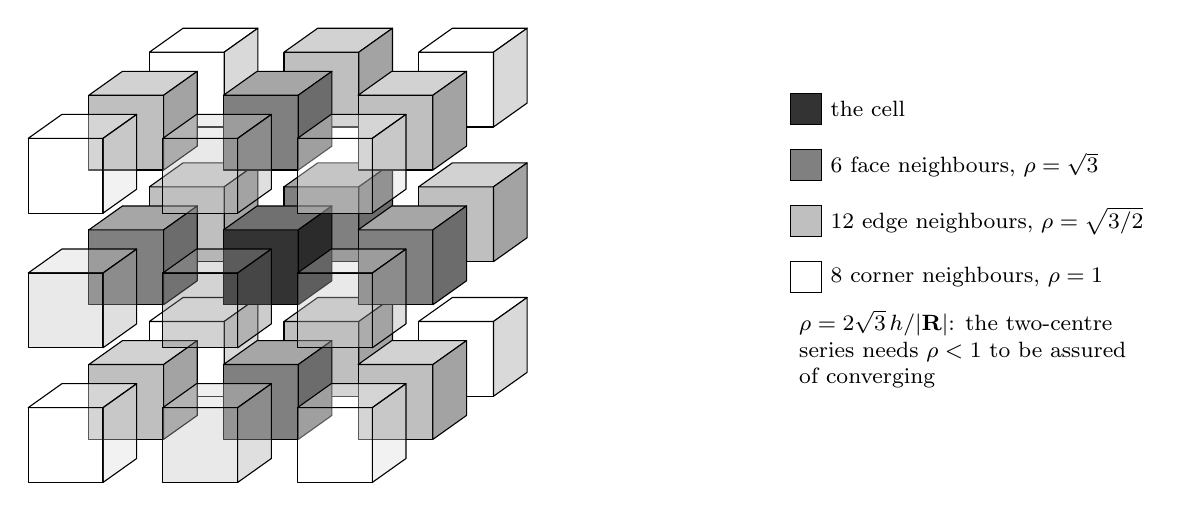
\begin{tikzpicture}[x=0.95cm, y=0.95cm, font=\footnotesize]
  \def\gap{1.8}
  \foreach \j in {1,0,-1}{
    \foreach \k in {-1,0,1}{
      \foreach \i in {-1,0,1}{
        \pgfmathtruncatemacro{\kind}{abs(\i) + abs(\j) + abs(\k)}
        \pgfmathsetmacro{\x}{\gap*\i}
        \pgfmathsetmacro{\y}{\gap*\j}
        \pgfmathsetmacro{\z}{\gap*\k}
        % the nine cubes of the front layer are drawn see-through, so the cell behind them shows
        \ifnum\j<0 \renewcommand{\cubeopacity}{0.35}\else\renewcommand{\cubeopacity}{1}\fi
        \ifcase\kind
          \cube{\x}{\y}{\z}{centre}
        \or
          \cube{\x}{\y}{\z}{face}
        \or
          \cube{\x}{\y}{\z}{edge}
        \or
          \cube{\x}{\y}{\z}{corner}
        \fi
      }
    }
  }
  % legend
  \begin{scope}[xshift=7.2cm, yshift=3.0cm]
    \foreach \col/\lab [count=\r] in {centre/{the cell},
        face/{6 face neighbours, $\rho=\sqrt3$},
        edge/{12 edge neighbours, $\rho=\sqrt{3/2}$},
        corner/{8 corner neighbours, $\rho=1$}}{
      \filldraw[fill=\col, draw=black, thin] (0,-0.75*\r) rectangle ++(0.42,0.42);
      \node[right, inner sep=3pt] at (0.42,-0.75*\r+0.21) {\lab};
    }
    \node[right, align=left, inner sep=3pt] at (0,-3.75) {$\rho=2\sqrt3\,h/|\mathbf R|$: the two-centre\\
      series needs $\rho<1$ to be assured\\ of converging};
  \end{scope}
\end{tikzpicture}
\end{document}
